\documentclass[12pt,a4paper]{article}
\usepackage[T2A]{fontenc}
\usepackage[utf8]{inputenc}
\usepackage[russian]{babel}
\usepackage{graphicx, setspace, hyperref, fontspec}
\setmainfont{Merriweather}

\usepackage[
top = 1.25cm, 
bottom = 2.0cm]{geometry}

\begin{document}
\begin{titlepage} 
	\centering
    % HEADER
	{
        \scshape
        Федеральное государственное автономное образовательное учреждение высшего образования
        \par
        \textbf{«Научно-образовательная корпорация ИТМО»}
        \par
        \vspace{1cm}
        Факультет Программной Инженерии и Компьютерной Техники
        \par
    }
    % LOGO
    \vspace{0.6cm}
    
\includegraphics[width=\textwidth]{logo.png}
    % LAB INFO
    {
        \Large
        \textbf{Лабораторная работа №1 по основам программной инженерии}
        \par
        \normalsize
        \vspace{0.75cm}
        \textbf{Вариант 3174}
        \par
    }
    \vfill
    % СREDITS
    \hfill\begin{minipage}{\dimexpr\textwidth-7.8cm}
        \textbf{Выполнил:}\par
        Степанов Арсений Алексеевич\par
        Шпак Всеволод Васильевич\par
        \vspace{0.15cm}
        \textbf{Группа:}\par
        P3209\par
        \vspace{0.15cm}
        \textbf{Преподаватель:}\par
        Пименов Данила Дмитриевич\par
    \end{minipage}
    \vfill
    Санкт-Петербург, \the\year{}г
\end{titlepage}  
\section{Задание}
Составить список требований, предъявляемых к разрабатываемому веб-сайту (\href{http://duckduckgo.com}{duckduckgo.com}). Требования должны делиться на следующие категории:
\begin{itemize}
    \item Функциональные
    \begin{itemize}
        \item Требования пользователей сайта
        \item Требования владельцев сайта
    \end{itemize}
    \item Нефункциональные
\end{itemize}
Требования необходимо оформить в соответствии с шаблонами RUP (документ SRS - Software Requirements Specification). Для каждого из требований нужно указать его атрибуты (в соответствии с методологией RUP), а также оценить и аргументировать приблизительное количество часов, требующихся на реализацию этого требования. \\
\\
Для функциональных требований нужно составить UML UseCase-диаграммы, описывающие реализующие их прецеденты использования
\part*{Спецификация требований к программному обеспечению}
\section{Введение}
\subsection{Цель}
Сайт DuckDuckGo используется в качестве поисковой системы, ориентированной на приватность пользователей. В отличие от многих других поисковых систем, DuckDuckGo не сохраняет историю поиска пользователей и не профилирует их с целью таргетирования рекламы. Это делает его предпочтительным выбором для тех, кто стремится к более конфиденциальному взаимодействию в интернете
\subsection{Соглашения о терминологии внутри проекта}
\begin{itemize}
    \item Бекенд: Часть программного обеспечения, работающая на сервере. Она обрабатывает запросы поиска, индексацию веб-страниц и подготавливает результаты поиска для фронтенда
    \item Библиотека: Коллекция предопределённого функционала, которую можно использовать для расширения возможностей поисковика или упрощения разработки
    \item Фреймворк: Набор инструментов и библиотек, облегчающих создание и поддержку поисковой системы, предоставляя готовую структуру для разработки
    \item Фронтенд: Пользовательский интерфейс поисковика, с которым напрямую взаимодействуют пользователи. Включает в себя элементы управления и отображение результатов поиска
    \item CSS (Cascading Style Sheets): Язык стилей для определения внешнего вида веб-страниц, в том числе страниц результатов поиска DuckDuckGo
    \item HTML (HyperText Markup Language): Язык разметки для структурирования контента на веб-страницах, включая страницы результатов поиска DuckDuckGo
    \item JS (JavaScript): Язык программирования для создания интерактивных элементов на веб-страницах, используемый в DuckDuckGo для улучшения пользовательского опыта
    \item Политика конфиденциальности: Правила и условия, обеспечивающие защиту личных данных пользователей DuckDuckGo
    \item Tor: Сеть для анонимного взаимодействия в интернете, поддержка которой встроена в DuckDuckGo, позволяя пользователям обеспечивать ещё большую конфиденциальность
    \item Software Requirements Specification (SRS): Документ, описывающий все функциональные и нефункциональные требования к программному продукту
    \item UseCase (Сценарий использования): Описание последовательности действий, выполняемых системой, для достижения конкретной цели пользователя

\end{itemize}
\subsection{Целевая аудитория}
Целевая аудитория сайта DuckDuckGo - пользователи интернета, которые заинтересованы в сохранении своей приватности при поиске информации в сети. Это включает в себя широкий спектр пользователей, от обычных людей, искренне обеспокоенных защитой своих персональных данных, до профессионалов и компаний, стремящихся обезопасить свою коммерческую информацию
\subsection{Объём проекта}
Средний масштаб проекта: DuckDuckGo является меньшим по сравнению с крупнейшими поисковыми системами
\section{Общее описание}
\subsection{Особенности продукта}
В данном разделе представлен обзор ключевых функций DuckDuckGo, включая:
\begin{itemize}
    \item Поиск без отслеживания: DuckDuckGo не сохраняет личную информацию пользователей и не отслеживает их поисковую историю
    \item Быстрые ответы: Предоставляет мгновенные ответы на общие вопросы прямо в результатах поиска
    \item !bang команды: Позволяют пользователям напрямую искать на тысячах других сайтов, вводя соответствующие команды
    \item Тематические инстанс-ответы: Показывает специфическую информацию по запросам, например, прогноз погоды или результаты спортивных матчей
    \item Поддержка анонимности через Tor: Обеспечивает дополнительный уровень приватности для пользователей, использующих сеть Tor
\end{itemize}
\subsection{Окружающая среда эксплуатации}
DuckDuckGo разработан для работы в разнообразных операционных системах через веб-браузеры и доступен в виде мобильных приложений для iOS и Android. Продукт требует подключения к интернету
\subsection{Ограничения проектирования и реализации}
\begin{itemize}
    \item Языки программирования: Использование различных языков программирования для фронтенда и бекенда, включая JavaScript и Python
    \item Стандарты кодирования: Применяются общепринятые стандарты написания кода для обеспечения высокого качества кода
    \item Совместимость: Продукт разрабатывается с учетом совместимости с последними версиями основных браузеров и операционных систем
    \item Конфиденциальность: Строгое соблюдение политик конфиденциальности во всех аспектах разработки и эксплуатации поисковика
\end{itemize}
\subsection{Документация для пользователей}
Для DuckDuckGo предусмотрены следующие виды документации для пользователей:
\begin{itemize}
    \item Руководства пользователя: Подробные инструкции по использованию поисковика и его уникальных функций
    \item Часто задаваемые вопросы (FAQ): Раздел с ответами на общие вопросы пользователей
    \item Видеоуроки: Обучающие видео, покрывающие ключевые функции и рекомендации по использованию DuckDuckGo
    \item Сообщество и форум поддержки: Платформа для обмена знаниями и решения вопросов среди пользователей
    \item Блог: Статьи с советами, руководствами и новостями о последних обновлениях и функциях DuckDuckGo
\end{itemize}
\subsection{Предположения и зависимости}
\subsubsection{Предположения}
\begin{itemize}
    \item Пользователи заинтересованы в приватности и безопасности своих данных в интернете
    \item Пользователи имеют доступ к интернету и используют поддерживаемые веб-браузеры и операционные системы
\end{itemize}
\subsubsection{Зависимости}
\begin{itemize}
    \item Эффективность поиска и скорость загрузки результатов зависят от инфраструктуры, на которой размещен DuckDuckGo
    \item Постоянное обновление и улучшение функций поиска требуют постоянной работы команды разработчиков и адаптации к изменяющимся технологиям и трендам в области поисковых систем и интернет-безопасности
\end{itemize}
\section{Функциональные требования}
\subsection{Для пользователей}
\begin{itemize}
    \item U1: Пользователи могут осуществлять поиск в интернете через DuckDuckGo без отслеживания истории поиска и собирания личных данных
    \item U2: Предоставляется возможность получать быстрые ответы на общие вопросы прямо в результатах поиска
    \item U3: Возможность использования !bang команд для быстрого перехода к поиску на других сайтах прямо из DuckDuckGo
    \item U4: Система показывает тематические инстанс-ответы, например, прогнозы погоды или результаты спортивных событий, в зависимости от запроса пользователя
    \item U5: Пользователям доступны настройки для персонализации поискового опыта, включая изменение тем оформления и конфигурации приватности
    \item U6: Предусмотрена возможность использования DuckDuckGo через Tor для обеспечения дополнительной анонимности поиска
    \item U7: Пользователи могут делиться результатами поиска через различные социальные сети с помощью специальных ссылок
    \item U8: Система поддерживает добавление DuckDuckGo в браузер в качестве поисковой системы по умолчанию
    \item U9: Предоставляется доступ к обширной базе данных с ответами на часто задаваемые вопросы о работе поисковика и приватности в интернете
    \item U10: Возможность сохранения предпочтений поиска и настроек приватности в профиле пользователя без необходимости регистрации
\end{itemize}
\subsection{Для владельцев}
\begin{itemize}
    \item O1: Владельцы имеют доступ к аналитическим инструментам для мониторинга общего использования поисковика
    \item O2: Возможность обновления и добавления новых функций и сервисов без прерывания работы поисковика
    \item O3: Управление рекламными кампаниями в рамках поисковика с соблюдением принципов приватности
\end{itemize}
\section{Нефункциональные требования}
\subsection{Требования к удобству использования}
\begin{itemize}
    \item N1: Интуитивно понятный и простой интерфейс, поддерживающий эффективный поиск и доступ к функциям поисковика
    \item N2: Поддержка адаптивного дизайна для комфортного использования на различных устройствах и разрешениях экрана
\end{itemize}
\subsection{Требования к производительности}
\begin{itemize}
    \item N3: Быстрая загрузка результатов поиска
    \item N4: Поддержка высокого объема запросов без снижения скорости и качества работы поисковика
\end{itemize}
\subsection{Требования к безопасности}
\begin{itemize}
    \item N5: Использование современных методов шифрования и защиты данных для обеспечения безопасности поиска и пользовательских настроек
    \item N6: Регулярное обновление программного обеспечения для предотвращения уязвимостей безопасности
\end{itemize}
\subsection{Требования к качеству программного обеспечения}
\begin{itemize}
    \item N7: Постоянное тестирование и обновление поисковика для улучшения функциональности и устранения ошибок
    \item N8: Обеспечение высокой доступности и надежности сервиса
\end{itemize}
\subsection{Требования к внешним интерфейсам}
\begin{itemize}
    \item N9: Предоставление API для интеграции с другими сервисами и приложениями, обеспечивая возможность использования функций поисковика в сторонних продуктах
    \item N10: Мультиязычная поддержка интерфейса и документации, облегчающая доступ к поисковику для пользователей всего мира
\end{itemize}
\section{Анализ временных затрат}
\begin{itemize}
    \item U1: Неотслеживаемый поиск - 200-300 часов. Разработка приватного механизма поиска требует создания специальной архитектуры и защиты данных
    \item U2: Быстрые ответы - 150-200 часов. Необходимо интегрировать и оптимизировать базу данных для быстрых ответов и реализовать логику их выбора
    \item U3: !Bang команды - 100-150 часов. Требуется создать и поддерживать обширную базу команд и управлять перенаправлениями запросов
    \item U4: Инстанс-ответы - 200-250 часов. Сложность в интеграции разнообразных источников данных и форматировании ответов под запросы
    \item U5: Персонализация настроек - 150-200 часов. Разработка интерфейса пользователя и механизма сохранения настроек без регистрации
    \item U6: Поддержка Tor - 50-100 часов. Интеграция с Tor для анонимного доступа к поиску
    \item U7: Поделиться результатами - 40-80 часов. Реализация функции создания и распространения специальных ссылок
    \item U8: Добавление в браузер - 20-40 часов. Создание простого способа установки DuckDuckGo как поисковой системы по умолчанию
    \item U9: База данных FAQ - 100-150 часов. Составление, форматирование и интеграция обширной базы знаний
    \item U10: Сохранение настроек - 100-200 часов. Разработка безопасного и удобного механизма сохранения настроек в профиле
    \item O1: Аналитические инструменты - 150-250 часов. Создание инструментов аналитики с соблюдением приватности
    \item O2: Обновление функций - 200-300 часов. Разработка архитектуры, позволяющей легко добавлять и обновлять функционал
    \item O3: Управление рекламой - 100-150 часов. Интеграция системы управления рекламой с учетом приватности
    \item N1: Удобный интерфейс - 200-300 часов. Дизайн и тестирование пользовательского интерфейса для удобства использования
    \item N2: Адаптивный дизайн - 150-200 часов. Разработка и тестирование дизайна, который корректно работает на разных устройствах
    \item N3: Быстрая загрузка - 100-200 часов. Оптимизация производительности для обеспечения быстрой загрузки результатов
    \item N4: Поддержка запросов - 250-350 часов. Масштабирование системы для обработки высокого объема запросов
    \item N5: Защита данных - 200-300 часов. Реализация современных методов защиты данных и шифрования
    \item N6: Обновление безопасности - 100-200 часов. Разработка и внедрение системы регулярных обновлений безопасности
    \item N7: Тестирование и обновление - 250-400 часов. Непрерывное тестирование и обновление функциональности для устранения ошибок
    \item N8: Доступность сервиса - 200-300 часов. Обеспечение стабильности и надежности работы сервиса
    \item N9: API для интеграции - 150-250 часов. Разработка и документирование API для сторонних разработчиков
    \item N10: Интернационализация - 100-200 часов. Перевод интерфейса и документации на разные языки
\end{itemize}
\part*{Риски}
\section{Прямые риски}
\textbf{Технологические ограничения:} Разработчики и проектные менеджеры сталкиваются с ограничениями существующих веб-технологий, которые могут не позволить реализовать некоторые функции, включая анонимный поиск в интернете через DuckDuckGo без отслеживания и сбора личных данных (U1). Это может уменьшить общую функциональность поисковика, влияя на удовлетворенность пользователей и их доверие к сервису
\\ \hfill\break
Вероятность возникновения: 1\% \\
Потенциальные потери: Высокие

\section{Непрямые риски}
\textbf{Изменения в предпочтениях пользователей и появление новых технологий:} Команда по исследованию и разработке (ИР) может столкнуться с трудностями из-за нововведений в технологиях и изменений в предпочтениях пользователей, что может сделать текущие требования к дизайну и удобству использования (N1, N2) менее актуальными. Это потребует от команды быстрой адаптации системы, чтобы оставаться конкурентоспособной на рынке
\\ \hfill\break
Вероятность возникновения: 0.6\% \\
Потенциальные потери: Средние

\section{Ресурсные риски}
\textbf{Недостаток квалифицированных специалистов:} HR-отдел и руководство проекта могут столкнуться с проблемой найма опытных разработчиков, что затруднит реализацию сложных функций, таких как предоставление быстрых ответов на общие вопросы (U2) и сохранение настроек приватности без регистрации (U10). Это может замедлить процесс разработки и увеличить его стоимость
\\ \hfill\break
Вероятность возникновения: 2\% \\
Потенциальные потери: Высокие

\subsection{Финансовые ограничения}
Ограниченный бюджет, с которым сталкивается финансовый отдел, может привести к урезанию критически важных функций, что скажется на скорости загрузки результатов поиска (N3) и способности системы обрабатывать высокий объем запросов (N4). Это может негативно отразиться на конкурентоспособности продукта
\\ \hfill\break
Вероятность возникновения: 2\% \\
Потенциальные потери: Высокие

\section{Бизнес риски}
\subsection{Неприятие рынком}
Отдел маркетинга и продуктовые менеджеры могут столкнуться с риском, что внедряемые функциональные возможности, такие как тематические инстанс-ответы (U4) и персонализация поискового опыта (U5), не найдут отклика у целевой аудитории, что затруднит достижение целей по привлечению и удержанию пользователей
\\ \hfill\break
Вероятность возникновения: 2\% \\
Потенциальные потери: Высокие

\subsection{Конкуренция}
Команда стратегического планирования и анализа конкурентов может обнаружить, что быстрая адаптация конкурентами аналогичных или превосходящих решений снижает привлекательность собственного продукта на рынке, что требует поиска новых стратегий для сохранения конкурентного преимущества
\\ \hfill\break
Вероятность возникновения: 5\% \\
Потенциальные потери: Средние

\section{Технические риски}
\textbf{Риск возникновения ошибок:} Команда разработчиков и QA-специалисты могут столкнуться с повышенным риском возникновения ошибок из-за сложности реализаций некоторых функций, таких как механизмы быстрых ответов (U2) и современные методы шифрования (N6). Это требует повышенных усилий на тестирование и обеспечение качества, что может также повлечь увеличение времени и затрат на разработку
\\ \hfill\break
Вероятность возникновения: 3\% \\
Потенциальные потери: Маленькие

\section{Политические риски}
\textbf{Законодательные ограничения:} Юридический отдел и специалисты по соответствию стандартам могут столкнуться с ограничениями, налагаемыми различными законодательными рамками по странам, что может ограничить использование определённых функций, таких как алгоритмы шифрования (N6) и возможности поиска через Tor для усиления анонимности (U6)
\\ \hfill\break
Вероятность возникновения: 0.5\% \\
Потенциальные потери: Средние

\section{Форс-мажор}
\textbf{Непредвиденные обстоятельства:} Команда управления проектом и руководство компании должны быть готовы к непредвиденным обстоятельствам, таким как природные катастрофы, пандемии или кибератаки, которые могут серьезно нарушить разработку и поддержку поисковой системы, затрагивая все аспекты проекта от разработки до доступности сервиса
\\ \hfill\break
Вероятность возникновения: 0.3\% \\
Потенциальные потери: Высокие

\part*{UseCase}
\begin{center}
    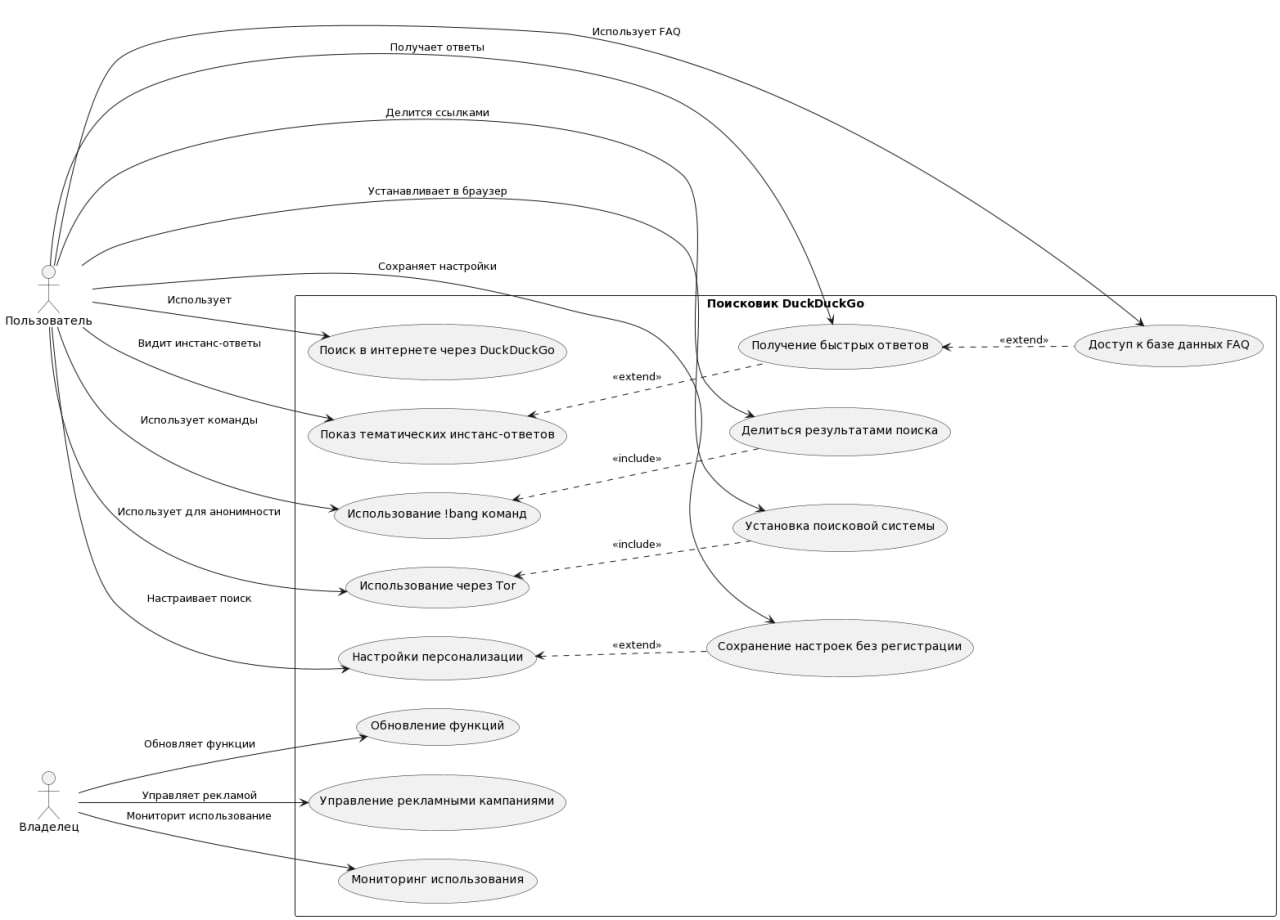
\includegraphics[width=\textwidth]{usecase.jpg}
\end{center}
\part*{Прототип интерфейса}
\section{Пользовательские интерфейсы}
\begin{itemize}
    \item Главная страница: Простой и чистый интерфейс с полем поиска в центре, предлагающий конфиденциальность без отслеживания поисковой активности пользователя
    \item Страница результатов поиска: Отображает результаты поиска без персонализации, основываясь исключительно на введенном запросе, с возможностью фильтрации по видео, изображениям, новостям и т.д
    \item Настройки поиска: Позволяют пользователям настраивать внешний вид поисковой системы, включая темы, язык и конфигурации приватности
    \item Страницы помощи и поддержки: Предоставляют информацию о функциях поисковой системы, настройках приватности и часто задаваемых вопросах
    \item Страница настроек приватности: Предлагает различные уровни настройки приватности и информацию о том, как DuckDuckGo обеспечивает защиту данных пользователя
\end{itemize}
\section{Аппаратные интерфейсы}
\begin{itemize}
    \item Серверная инфраструктура: Распределенная серверная инфраструктура для обработки запросов поиска с высокой доступностью и надежностью
    \item Балансировщики нагрузки: Используются для распределения трафика поиска по серверам, оптимизируя время отклика и производительность
    \item Защита от DDoS-атак: Специализированные системы для обнаружения и смягчения DDoS-атак для обеспечения непрерывности сервиса.    
\end{itemize}
\section{Программные интерфейсы}
\begin{itemize}
    \item Микросервисная архитектура: Использование микросервисов для обеспечения масштабируемости и упрощения разработки и обслуживания различных компонентов системы
    \item API для интеграции: Предоставляет API для разработчиков, позволяя интегрировать функции поиска DuckDuckGo в сторонние приложения и сервисы
    \item Защищенное хранение данных: Использование зашифрованного хранения для обеспечения безопасности данных пользователей и запросов
\end{itemize}
\section{Сетевые интерфейсы}
\begin{itemize}
    \item HTTPS для всех запросов: Все запросы к DuckDuckGo проходят через HTTPS, обеспечивая конфиденциальность и безопасность данных пользователей
    \item CDN (Сеть доставки контента): Использование CDN для быстрой и эффективной доставки контента пользователям по всему миру, снижая задержку и ускоряя загрузку страниц
    \item VPC (Виртуальные частные сети): Защищенные виртуальные частные сети для внутренней коммуникации между сервисами и инфраструктурой, обеспечивающие безопасность данных и операций
\end{itemize}
\part*{Вывод}
В рамках выполнения этой лабораторной работы произошло знакомство с принципами методологии RUP и форматом документа SRS. Была разработана UML UseCase-диаграмма, а также подготовлен и оформлен список требований к веб-сайту в соответствии со стандартами SRS
\end{document}